\documentclass{beamer}
%use the theme Copenhagen
\usetheme{Copenhagen}
%to set the language Russian
\usepackage[utf8]{inputenc}
\usepackage[T2A]{fontenc}
\usepackage[russian]{babel}
%to adjust the width of the table
\usepackage{array}  
% Adjust the margin here
\setbeamersize{text margin left=0.3cm, text margin right=0.3cm} 
%Add package command to adjustment page
\usepackage{changepage}  
%Information to be included in the title page:
\title{\textbf{Необязательное задание №2}}
\author{ФИО: \textbf{Фам} Данг Чунг \textbf{Нгиа}}
\date{Номер варианта= $1+((3*4) mod 8)=\textbf{5}$}

\logo{
\includegraphics[width=2.2cm]{Logo.png}}


\begin{document}
%set the  title page
\frame{\titlepage}
\begin{frame}{Перевод из одной СС в другую. Пример 1}
    \small{
$231_{(10)}=ABC_{(10)}=...HGFE_{(8)}=...+H*8^{3}+G*8^{2}+F*8+E$, при натуральных $H, G, F ,E<8$,\par
\begin{center}
        Как найти E, F, G, H?
\end{center}
Решение: $(...+H*8^{3}+G*8^{2}+F*8+E)/8= ...+H*8^{2}+G*8^{1}+F$ (плюс остаток E) => $(...HGFE_{(8)})/8=...HGF_{(8)}$ (с остатком E)\\
\begin{center}
    \begin{tabular}{|c|c|c|c|c|c|c|}
    \hline
        Номер шага (i) & 0 & 1 & 2 & 3 & 4 & ...\\
        \hline
        Частное от деления на 8 & 231 & 28 & 3 & 0 & 0 & 0\\
        \hline
        Остаток от деления на 8 & 0 & 7 & 4 & 3 & 0 & 0\\
        \hline
    \end{tabular}
    \vspace{1em}
        
    Ответ: E=7, F=4, G=3, H=0.\\
    $231_{(10)}=347_{(8)}$
\end{center}
}

\end{frame}


\begin{frame}{Перевод из одной СС в другую. Пример 3}
    \small{
Задача: $0,15_{(10)}=?_{(3)}=0,ABCD..._{(3)}=A/3^{1}+B/3^{2}+C/3^{3}+D/3^{4}+...$\\
Решение: $(A/3^{1}+B/3^{2}+C/3^{3}+D/3^{4}+...)*3=A*3^{0}+(B/3^{1}+C/3^{2}+D/3^{4}+...)=>3*0,ABCD..._{(3)}=A,BCD..._{(3)}$\\

\begin{tabular}{| m{5cm} | m{0.5cm} | m{0.5cm} | m{0.5cm} | m{0.5cm} | m{0.5cm} | m{0.5cm} | m{0.5cm} |}
    \hline
    Номер шага (\textit{i}) & 0 & 1 & 2 & 3 & 4 & 5 & ... \\
    \hline
    Целая часть после умножения дробной части на 3 & 0 & 0 & 1 & 1 & 0 & 0 & ...\\
    \hline
    Дробная часть после умножения на 3 & 0,15 & 0,45 & 0,35 & 0,05 & 0,15 & 0,45 & ...\\
    \hline
\end{tabular}
Ответ: $0,15_{(10)}= 0,011001100..._{(3)}=0,(0110)_{(3)}$
}


 

\end{frame}

\begin{frame}{Преобразование из CC-2 в CC-$2^{k}$ и обратно}
    \begin{tabular}{|m{3.5cm}|m{3.5cm}|m{3.5cm}|}
\hline
    \textbf{\scriptsize{Двоичная <-> Четверичная}} & \textbf{\scriptsize{Двоичная <-> Восьмеричная}} & \textbf{\scriptsize{Двоичная <-> Шестнадцатеричная}}\\
    \hline
    00 <-> 0 & 000 <-> 0 & 0000 <-> 0 \\
    \hline
    01 <-> 1 & 001 <-> 1 & 0001 <-> 1 \\
    \hline
    10 <-> 2 & 010 <-> 2 & 0010 <-> 2 \\
    \hline
    11 <-> 3 & 011 <-> 3 & 0011 <-> 3 \\
    \hline
    & 100 <-> 4 & ... \\
    \hline
    & 101 <-> 5 & 1101 <-> D \\
    \hline
    & 110 <-> 6 & 1110 <-> E \\
    \hline
    & 111 <-> 7 & 1111 <-> F \\
    \hline
\end{tabular}
Пример: $1111110001,1110001_{(2)} = 0011 1111 0001,1110 0010_{(2)} = 3F1,E2_{(16)}$

\end{frame}

\begin{frame}{Преобразование из CC-N в CC-$N^{k}$ и обратно}
    \small{
\textbf{Из СС-N в СС-$N^{k}$}\\
\textbullet\quadдополнить число, записанное в СС с основанием N, незначащими нулями так, чтобы количество цифр было кратно k;\\
\textbullet\quad разбить полученное число на группы по k цифр, начиная от нуля;\\
\textbullet\quad заменить каждую такую группу эквивалентным числом, записанным в СС с основанием $N^{k}$.\\
\begin{adjustwidth}{1cm}{0cm}
    Задача: $1020101_{(3)} = ?_{(27)}$\\
    Решение: $1020101_{(3)} = 001 020 101_{(3)} = 16A?_{(27)}$\\
\end{adjustwidth}
\textbf{Из СС-$N^{k}$ в СС-N}\\
\textbullet\quad заменить каждую цифру числа, записанного в CC с основанием $N^{k}$, эквивалентным набором из k цифр CC с основанием N.\\
\begin{adjustwidth}{1cm}{0cm}
    Задача: $2345_{(125)} = ?_{(5)}$\\
Решение: $2345_{(125)} = 002 003 004 010_{(5)} = 2003004010_{(5)}$
\end{adjustwidth}
}
\end{frame}

\begin{frame}{Оптимальная система счисления}
    \small{\textbf{Задача.} Робинзон Крузо нашёл на острове 60 камней. Сколько прошедших дней можно ими закодировать в разных СС?\\
\textbf{Пример СС-10:}\\
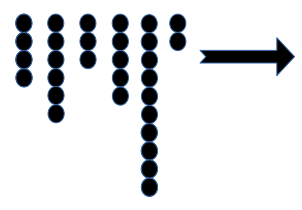
\includegraphics[width=2cm]{photo1_dop2.png}
463502-й день из 999999 возможных, где $999999 = 10^{6} - 1$\\
\begin{flushright}
    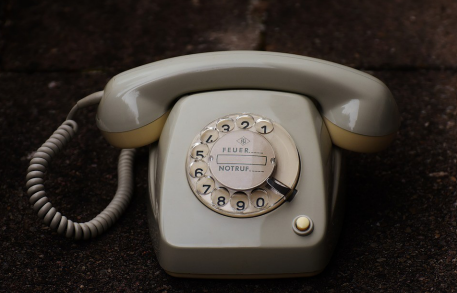
\includegraphics[width=4cm]{photo2_dop2.png}
\end{flushright}

}
\end{frame}
\end{document}